\documentclass[10pt,border=2pt]{standalone}
\usepackage[T1]{fontenc}
\usepackage{lmodern}
\usepackage{pgfplots}
\pgfplotsset{compat=1.18}
\definecolor{convexblue}{HTML}{0072B2}
\definecolor{concaveorange}{HTML}{D55E00}
\begin{document}
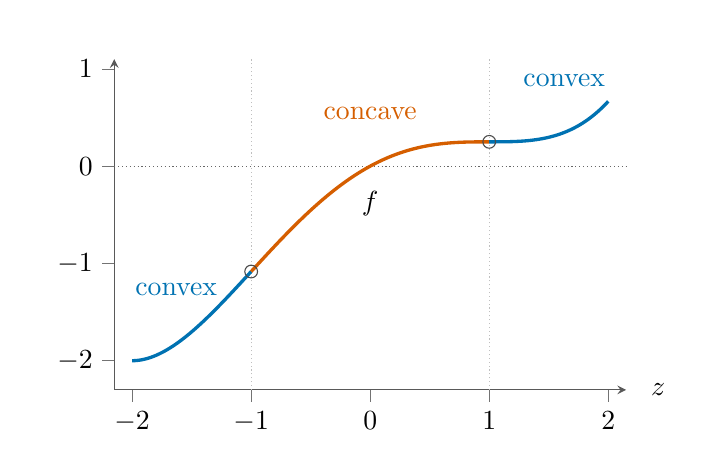
\begin{tikzpicture}
\path[use as bounding box] (-1.1,-0.65) rectangle (7.1,4.6);
\begin{axis}[
  scale only axis,width=6.5cm,height=4.2cm,
  at={(0,0)},anchor=south west,
  xmin=-2.15,xmax=2.15,xtick={-2,-1,0,1,2},
  ymin=-2.3,ymax=1.1,ytick={-2,-1,0,1},
  axis lines=left,axis line style={black!65},
  tick align=outside,tick style={black!55},
  xlabel={$z$},xlabel style={at={(axis description cs:1.03,0)},anchor=west},
  label style={font=\normalsize},tick label style={font=\normalsize},
  clip=false,
]
\addplot[black!60,densely dotted,thin] coordinates {(-2.15,0) (2.15,0)};
\addplot[black!25,densely dotted,thin] coordinates {(-1,-2.3) (-1,1.1)};
\addplot[black!25,densely dotted,thin] coordinates {(1,-2.3) (1,1.1)};
\addplot[convexblue,very thick,domain=-2:-1,samples=81] {x^4/12-x^2/2+2*x/3};
\addplot[concaveorange,very thick,domain=-1:1,samples=121] {x^4/12-x^2/2+2*x/3};
\addplot[convexblue,very thick,domain=1:2,samples=81] {x^4/12-x^2/2+2*x/3};
\addplot[only marks,mark=o,mark options={fill=white},mark size=2.3pt,black!70]
  coordinates {(-1,-1.083333333333) (1,0.25)};
\node[convexblue,anchor=south] at (axis cs:-1.63,-1.43) {convex};
\node[convexblue,anchor=south] at (axis cs:1.63,0.72) {convex};
\node[concaveorange,anchor=south] at (axis cs:0,0.38) {concave};
\node[anchor=north] at (axis cs:0,-0.16) {$f$};
\end{axis}
\end{tikzpicture}
\end{document}
